%-------------------------
% Resume in Latex
% Author : Jake Gutierrez
% Based off of: https://github.com/sb2nov/resume
% License : MIT
%------------------------

\documentclass[letterpaper,11pt]{article}

\usepackage{latexsym}
\usepackage[empty]{fullpage}
\usepackage{titlesec}
\usepackage{marvosym}
\usepackage[usenames,dvipsnames]{color}
\usepackage{verbatim}
\usepackage{enumitem}
\usepackage[hidelinks]{hyperref}
\usepackage{fancyhdr}
\usepackage[english]{babel}
\usepackage{tabularx}
\usepackage{tikz}
\input{glyphtounicode}


%----------FONT OPTIONS----------
% sans-serif
% \usepackage[sfdefault]{FiraSans}
% \usepackage[sfdefault]{roboto}
% \usepackage[sfdefault]{noto-sans}
% \usepackage[default]{sourcesanspro}

% serif
% \usepackage{CormorantGaramond}
% \usepackage{charter}


\pagestyle{fancy}
\fancyhf{} % clear all header and footer fields
\fancyfoot{}
\renewcommand{\headrulewidth}{0pt}
\renewcommand{\footrulewidth}{0pt}

% Adjust margins
\addtolength{\oddsidemargin}{-0.5in}
\addtolength{\evensidemargin}{-0.5in}
\addtolength{\textwidth}{1in}
\addtolength{\topmargin}{-.5in}
\addtolength{\textheight}{1.0in}

\urlstyle{same}

\raggedbottom
\raggedright
\setlength{\tabcolsep}{0in}

% Sections formatting
\titleformat{\section}{
  \vspace{-4pt}\scshape\raggedright\large
}{}{0em}{}[\color{black}\titlerule \vspace{-5pt}]

% Ensure that generate pdf is machine readable/ATS parsable
\pdfgentounicode=1

%-------------------------
% Custom commands
\newcommand{\resumeItem}[1]{
  \item\small{
    {#1 \vspace{-2pt}}
  }
}

\newcommand{\resumeSubheading}[4]{
  \vspace{-2pt}\item
    \begin{tabular*}{0.97\textwidth}[t]{l@{\extracolsep{\fill}}r}
      \textbf{#1} & #2 \\
      \textit{\small#3} & \textit{\small #4} \\
    \end{tabular*}\vspace{-7pt}
}

\newcommand{\resumeSubSubheading}[2]{
    \item
    \begin{tabular*}{0.97\textwidth}{l@{\extracolsep{\fill}}r}
      \textit{\small#1} & \textit{\small #2} \\
    \end{tabular*}\vspace{-7pt}
}

\newcommand{\resumeProjectHeading}[2]{
    \item
    \begin{tabular*}{0.97\textwidth}{l@{\extracolsep{\fill}}r}
      \small#1 & #2 \\
    \end{tabular*}\vspace{-7pt}
}

\newcommand{\resumeSubItem}[1]{\resumeItem{#1}\vspace{-4pt}}

\renewcommand\labelitemii{$\vcenter{\hbox{\tiny$\bullet$}}$}

\newcommand{\resumeSubHeadingListStart}{\begin{itemize}[leftmargin=0.15in, label={}]}
\newcommand{\resumeSubHeadingListEnd}{\end{itemize}}
\newcommand{\resumeItemListStart}{\begin{itemize}}
\newcommand{\resumeItemListEnd}{\end{itemize}\vspace{-5pt}}

%-------------------------------------------
%%%%%%  RESUME STARTS HERE  %%%%%%%%%%%%%%%%%%%%%%%%%%%%


\begin{document}

%----------HEADING----------
% \begin{tabular*}{\textwidth}{l@{\extracolsep{\fill}}r}
%   \textbf{\href{http://sourabhbajaj.com/}{\Large Sourabh Bajaj}} & Email : \href{mailto:sourabh@sourabhbajaj.com}{sourabh@sourabhbajaj.com}\\
%   \href{http://sourabhbajaj.com/}{http://www.sourabhbajaj.com} & Mobile : +1-123-456-7890 \\
% \end{tabular*}

\begin{center}
    \textbf{\Huge \scshape Nurbek Khalmatay} \\ \vspace{1pt}
    \small +7(700)484-48-08 $|$ \href{khalmatay@gmail.com}{\underline{khalmatay@gmail.com}} $|$ 
    \href{https://linkedin.com/in/khalmatay}{\underline{linkedin.com/in/khalmatay}} $|$
    \href{https://github.com/Khalmatay}{\underline{github.com/Khalmatay}}
\end{center}


%-----------EDUCATION-----------
\section{Education}
  \resumeSubHeadingListStart
    \resumeSubheading
      {Satbayev University}{Almaty, Kazakhstan}
      {Bachelor of Computer Science GPA: 3.89/4.00}{Sep. 2021 - Jun 2024}
    \resumeItem{\textbf{Relevant coursework:}: Linear Algebra, Calculus, Probability Theory, Mathematical Statistics, Algorithms and data structures, Databases}
\resumeSubHeadingListEnd

%-----------EXPERIENCE-----------
\section{Experience}
  \resumeSubHeadingListStart
    \resumeSubheading
      {Spark Lab, Indrive}{Almaty, Kazakhstan}
      {Data Analyst Intern, Air Quality Monitoring team}{Jan. 2023 - May 2023}
       \resumeItemListStart
       \resumeItem{
       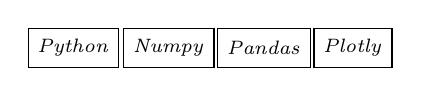
\begin{tikzpicture}
       \node[draw, shape=rectangle, minimum height=0.5cm, font=\scriptsize] at (0,0){\textit{Python}};
       \node[draw, shape=rectangle,minimum height=0.5cm, font=\scriptsize] at (1.21,0) {\textit{Numpy}};
       \node[draw, shape=rectangle, minimum height=0.5cm, font=\scriptsize] at (2.42,0) {\textit{Pandas}};
       \node[draw, shape=rectangle,minimum height=0.5cm, font=\scriptsize] at (3.55,0) {\textit{Plotly}};
       \end{tikzpicture}
       }
        \resumeItem{Developed \textbf{algorithms} that make it possible to identify vehicles with \textbf{a high probability of exceeding emission standards}. These algorithms are integrated into the eco-sensor system, which reduces the time for checking vehicles and increases the efficiency of eco-posts.}
        \resumeItem{Processed about \textbf{52,000 vehicles} and \textbf{84,000 eco-sensor records}. According to the results of the scoring, all cars were rated. The top \textbf{388 cars} (suspects) were transferred to Almaty Police Department (uploaded to tablets).}
        \resumeItem{Developed \textbf{interactive visualization of sorted data on the map} with data of date, time, number of cars near cameras and eco-sensors, PM 2.5 indicators.}
        \resumeItem{Trained by Sergek Group experts on how to study the subject area, ecology and air quality, the chemistry of fuel combustion, eco sensor, teamwork}
        
      \resumeItemListEnd
      
      
% -----------Multiple Positions Heading-----------
%    \resumeSubSubheading
%     {Software Engineer I}{Oct 2014 - Sep 2016}
%     \resumeItemListStart
%        \resumeItem{Apache Beam}
%          {Apache Beam is a unified model for defining both batch and streaming data-parallel processing pipelines}
%     \resumeItemListEnd
%    \resumeSubHeadingListEnd
%-------------------------------------------

    \resumeSubheading
      {Full-Stack Developer Summer Bootcamp, nFactorial Incubator}{Almaty, Kazakhstan}
      {Full Stack Developer}{Jun 2022 - Aug 2022}
      \resumeItemListStart
      \resumeItem{
       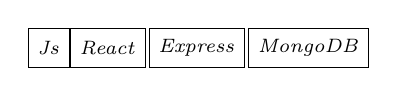
\begin{tikzpicture}
       \node[draw, shape=rectangle, minimum height=0.5cm, font=\scriptsize] at (0,0){\textit{Js}};
       \node[draw, shape=rectangle,minimum height=0.5cm, font=\scriptsize] at (0.75,0) {\textit{React}};
       \node[draw, shape=rectangle, minimum height=0.5cm, font=\scriptsize] at (1.88,0) {\textit{Express}};
       \node[draw, shape=rectangle,minimum height=0.5cm, font=\scriptsize] at (3.3,0) {\textit{MongoDB}};
       \end{tikzpicture}
       }
        \resumeItem{nFactorial Incubator is the largest tech Bootcamp \textbf{in Central Asia led by Princeton U graduate, FAANG engineers}.}\
        \resumeItem{10-week fullstack web development bootcamp program with \textbf{4.4\% acceptance rate} (181 out of 4071).}
        \resumeItem{Built a full-stack website to show what we learned for this summer using JavaScript, DOM, Events, JQuery, Bootstrap, NPM \& Local storag, React.JS, Lifecycle, useEffect, HTTP, JSON, MongoDB, Express.js}
        \resumeItem{Attended daily lectures and learned about how to build the website with React.js and how to write the Backend in JS, Node.js}
      \resumeItemListEnd
    
  \resumeSubHeadingListEnd


%-----------PROJECTS-----------
\section{Projects}
    \resumeSubHeadingListStart
      \resumeProjectHeading
          {\textbf{Gitlytics} $|$ \emph{Python, Flask, React, PostgreSQL, Docker}}{June 2020 -- Present}
          \resumeItemListStart
            \resumeItem{Developed a full-stack web application using with Flask serving a REST API with React as the frontend}
            \resumeItem{Implemented GitHub OAuth to get data from user’s repositories}
            \resumeItem{Visualized GitHub data to show collaboration}
            \resumeItem{Used Celery and Redis for asynchronous tasks}
          \resumeItemListEnd
      \resumeProjectHeading
          {\textbf{Simple Paintball} $|$ \emph{Spigot API, Java, Maven, TravisCI, Git}}{May 2018 -- May 2020}
          \resumeItemListStart
            \resumeItem{Developed a Minecraft server plugin to entertain kids during free time for a previous job}
            \resumeItem{Published plugin to websites gaining 2K+ downloads and an average 4.5/5-star review}
            \resumeItem{Implemented continuous delivery using TravisCI to build the plugin upon new a release}
            \resumeItem{Collaborated with Minecraft server administrators to suggest features and get feedback about the plugin}
          \resumeItemListEnd
    \resumeSubHeadingListEnd



%
%-----------PROGRAMMING SKILLS-----------
\section{Technical Skills}
 \begin{itemize}[leftmargin=0.15in, label={}]
    \small{\item{
     \textbf{Languages}{: Java, Python, C/C++, SQL (Postgres), JavaScript, HTML/CSS, R} \\
     \textbf{Frameworks}{: React, Node.js, Flask, JUnit, WordPress, Material-UI, FastAPI} \\
     \textbf{Developer Tools}{: Git, Docker, TravisCI, Google Cloud Platform, VS Code, Visual Studio, PyCharm, IntelliJ, Eclipse} \\
     \textbf{Libraries}{: pandas, NumPy, Matplotlib}
    }}
 \end{itemize}


%-------------------------------------------
\end{document}
